\documentclass{article}

\usepackage{fancyhdr}
\usepackage{extramarks}
\usepackage{amsmath}
\usepackage{amsthm}
\usepackage{amsfonts}
\usepackage{tikz}
\usepackage{tikz-qtree}
\usepackage[plain]{algorithm}
\usepackage{algpseudocode}
\usepackage{listings}
\usepackage{enumerate}
\lstset{breaklines=true}

\usetikzlibrary{automata,positioning,calc}

%
% Basic Document Settings
%

\topmargin=-0.45in
\evensidemargin=0in
\oddsidemargin=0in
\textwidth=6.5in
\textheight=9.0in
\headsep=0.25in

\linespread{1.1}

\pagestyle{fancy}
\lhead{\hmwkAuthorName}
\chead{\hmwkClass\ (\hmwkClassInstructor): \hmwkTitle}
\rhead{\firstxmark}
\lfoot{\lastxmark}
\cfoot{\thepage}

\renewcommand\headrulewidth{0.4pt}
\renewcommand\footrulewidth{0.4pt}

\setlength\parindent{0pt}

%
% Create Problem Sections
%

\newcommand{\enterProblemHeader}[1]{
    \nobreak\extramarks{}{Problem \arabic{#1} continued on next page\ldots}\nobreak{}
    \nobreak\extramarks{Problem \arabic{#1} (continued)}{Problem \arabic{#1} continued on next page\ldots}\nobreak{}
}

\newcommand{\exitProblemHeader}[1]{
    \nobreak\extramarks{Problem \arabic{#1} (continued)}{Problem \arabic{#1} continued on next page\ldots}\nobreak{}
    \stepcounter{#1}
    \nobreak\extramarks{Problem \arabic{#1}}{}\nobreak{}
}

\newcommand{\bipgraph}[2]{%
    \begin{tikzpicture}[every node/.style={circle,draw}]
    \foreach \xitem in {1,...,#1}
    {%
    % first set
    \node at (0,\xitem) (a\xitem) {};
    % second set
    \node at (2,\xitem) (b\xitem) {};   
    }%

    % connections
    \foreach \x [count=\xi] in {#2}
    {% 
    \foreach \tritem in \x % <-- Here no braces to make it a foreach list also not \xi but \x
    \draw(a\xi) -- (b\tritem);
    }
    \end{tikzpicture}  
}

\newcommand{\bipgraphComplete}[1]{%
    \begin{tikzpicture}[every node/.style={circle,draw}]
    \foreach \xitem in {1,...,#1}
    {%
    % first set
    \node at (0,\xitem) (a\xitem) {};
    % second set
    \node at (2,\xitem) (b\xitem) {};   
    }%

    % connections
    \foreach \x in {1,...,#1}
    {% 
    \foreach \y in {1,...,#1}
        \draw(a\x) -- (b\y);
    }
    \end{tikzpicture}  
}

\setcounter{secnumdepth}{0}
\newcounter{partCounter}
\newcounter{homeworkProblemCounter}
\setcounter{homeworkProblemCounter}{1}
\nobreak\extramarks{Problem \arabic{homeworkProblemCounter}}{}\nobreak{}

%
% Homework Problem Environment
%
% This environment takes an optional argument. When given, it will adjust the
% problem counter. This is useful for when the problems given for your
% assignment aren't sequential. See the last 3 problems of this template for an
% example.
%
\newenvironment{homeworkProblem}[1][-1]{
    \ifnum#1>0
        \setcounter{homeworkProblemCounter}{#1}
    \fi
    \section{Problem \arabic{homeworkProblemCounter}}
    \setcounter{partCounter}{1}
    \enterProblemHeader{homeworkProblemCounter}
}{
    \exitProblemHeader{homeworkProblemCounter}
}

%
% Homework Details
%   - Title
%   - Due date
%   - Class
%   - Section/Time
%   - Instructor
%   - Author
%

\newcommand{\hmwkTitle}{Homework\ \#4}
\newcommand{\hmwkDueDate}{February 11, 2015}
\newcommand{\hmwkClass}{Graph Theory}
\newcommand{\hmwkClassTime}{MWF 9:15}
\newcommand{\hmwkClassInstructor}{Professor McGinley}
\newcommand{\hmwkAuthorName}{Rick Sullivan}

%
% Title Page
%

\title{
    \vspace{2in}
    \textmd{\textbf{\hmwkClass:\ \hmwkTitle}}\\
    \normalsize\vspace{0.1in}\small{Due\ on\ \hmwkDueDate}\\
    \vspace{0.1in}\large{\textit{\hmwkClassInstructor\ \hmwkClassTime}}
    \vspace{3in}
}

\author{\textbf{\hmwkAuthorName}}
\date{}

\renewcommand{\part}[1]{\textbf{\large Part \Alph{partCounter}}\stepcounter{partCounter}\\}

%
% Various Helper Commands
%

% Useful for algorithms
\newcommand{\alg}[1]{\textsc{\bfseries \footnotesize #1}}

% For derivatives
\newcommand{\deriv}[1]{\frac{\mathrm{d}}{\mathrm{d}x} (#1)}

% For partial derivatives
\newcommand{\pderiv}[2]{\frac{\partial}{\partial #1} (#2)}

% Integral dx
\newcommand{\dx}{\mathrm{d}x}

% Alias for the Solution section header
\newcommand{\solution}{\textbf{\large Solution}}

% Probability commands: Expectation, Variance, Covariance, Bias
\newcommand{\E}{\mathrm{E}}
\newcommand{\Var}{\mathrm{Var}}
\newcommand{\Cov}{\mathrm{Cov}}
\newcommand{\Bias}{\mathrm{Bias}}

\begin{document}

\maketitle

\pagebreak

\begin{homeworkProblem}
    For which values of \(r\) is \(K_{r,r}\) Hamiltonian?
    \\

    \textbf{Solution}
    \\

    \bipgraphComplete{1}
    \bipgraphComplete{2}
    \bipgraphComplete{3}
    \bipgraphComplete{4}

    \(K_{r,r}\) is Hamiltonian for all \(r > 1\).
    Clearly there is no cycle on \(K_{1,1}\). 
    There exists a single Hamiltonian cycle on \(K_{2,2}\) for each vertex. 
    When we add 1 to \(r\) from a Hamiltonian complete bipartite graph, we can then include the two new vertices in the cycle because they are connected to every vertex in on the other side.
    Each successive graph is then also Hamiltonian.
\end{homeworkProblem}
\begin{homeworkProblem}
    Give an example of a graph with more than two vertices that is Hamiltonian but not Eulerian.
    \\

    \textbf{Solution}
    \\

    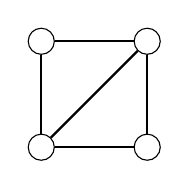
\begin{tikzpicture}[vertex/.style={circle,draw}]
        \node[vertex] (1) {};
        \node[vertex] (2) [right=1cm of 1] {};
        \node[vertex] (3) [below=1cm of 1] {};
        \node[vertex] (4) [right=1cm of 3] {};

        \path[draw,thick]
        (1) edge node {} (2)
        (1) edge node {} (3)
        (3) edge node {} (4)
        (2) edge node {} (4)
        (2) edge node {} (3);
    \end{tikzpicture}
\end{homeworkProblem}
\begin{homeworkProblem}
    Decide if the graph below is Hamiltonian. Explain your answer.
    \\

    \usetikzlibrary{shapes.geometric}
    \begin{tikzpicture}[vertex/.style={circle,draw,fill=black,inner sep=0pt,minimum size=5pt}]
        \node[draw=none, regular polygon, regular polygon sides=8, minimum size=2cm] (a) {};
        \node[draw,thick,regular polygon, regular polygon sides=8, minimum size=4cm] (b) {};

        \foreach \x in {1,...,8}{
            \node[vertex] at(a.corner \x) (a\x) {};
            \node[vertex] at(b.corner \x) (b\x) {};
        }

%\foreach[count=\i, evaluate=\i as \x using int(\i+6)] \y in {0,10,...,30}
        %\foreach[count=\i, evaluate=\i as \y using int(\i+2)] \x in {1,...,6}
        \foreach \a in {1,...,8} {
            \draw let \n1={int(mod(\a+1,8)+1)} in (a\a)--(a\n1);
        }

        % Edges joining concentric circles
        \foreach \x in {1,...,8}
            \draw (a\x)--(b\x);
    \end{tikzpicture}

    \textbf{Solution}
    \\

    Yes, the graph is Hamiltonian with the following cycle:

    \usetikzlibrary{shapes.geometric}
    \begin{tikzpicture}[vertex/.style={circle,draw,fill=black,inner sep=0pt,minimum size=5pt}]
        \node[draw=none, regular polygon, regular polygon sides=8, minimum size=2cm] (a) {};
        \node[draw,thick,regular polygon, regular polygon sides=8, minimum size=4cm] (b) {};

        \foreach \x in {1,...,8}{
            \node[vertex] at(a.corner \x) (a\x) {};
            \node[vertex] at(b.corner \x) (b\x) {};
        }

%\foreach[count=\i, evaluate=\i as \x using int(\i+6)] \y in {0,10,...,30}
        %\foreach[count=\i, evaluate=\i as \y using int(\i+2)] \x in {1,...,6}
        \foreach \a in {1,...,8} {
            \draw let \n1={int(mod(\a+1,8)+1)} in (a\a)--(a\n1);
        }

        % Edges joining concentric circles
        \foreach \x in {1,...,8}
            \draw (a\x)--(b\x);
    \end{tikzpicture}
\end{homeworkProblem}

\begin{homeworkProblem}
    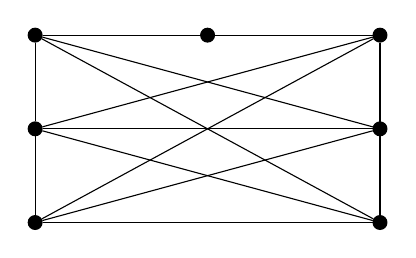
\begin{tikzpicture}[vertex/.style={circle,draw,fill=black,inner sep=0pt,minimum size=5pt}]
        \node[vertex] (a) {};
        \node[vertex] (b) [below=1cm of a] {};
        \node[vertex] (c) [below=1cm of b] {};
        \node[vertex] (g) [right=2cm of a] {};
        \node[vertex] (d) [right=2cm of g] {};
        \node[vertex] (e) [below=1cm of d] {};
        \node[vertex] (f) [below=1cm of e] {};

        \foreach \x in {b,d,e,f}{
            \draw (a)--(\x);
        }
        \foreach \x in {c,d,e,f}{
            \draw (b)--(\x);
        }
        \foreach \x in {d,e,f}{
            \draw (c)--(\x);
        }
        \draw (d)--(f);
    \end{tikzpicture}

    \textbf{Solution}
    \\

    We can divide the edges in the graph to create the following two cycles

    \(C1\)
    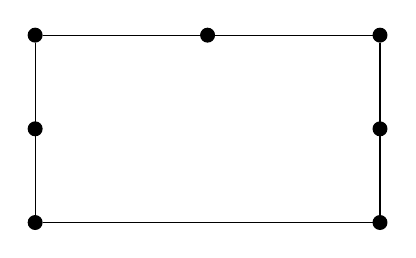
\begin{tikzpicture}[vertex/.style={circle,draw,fill=black,inner sep=0pt,minimum size=5pt}]
        \node[vertex] (a) {};
        \node[vertex] (b) [below=1cm of a] {};
        \node[vertex] (c) [below=1cm of b] {};
        \node[vertex] (g) [right=2cm of a] {};
        \node[vertex] (d) [right=2cm of g] {};
        \node[vertex] (e) [below=1cm of d] {};
        \node[vertex] (f) [below=1cm of e] {};

        \draw (a)--(d);
        \draw (a)--(c);
        \draw (c)--(f);
        \draw (d)--(f);
    \end{tikzpicture}
    \(C2\)
    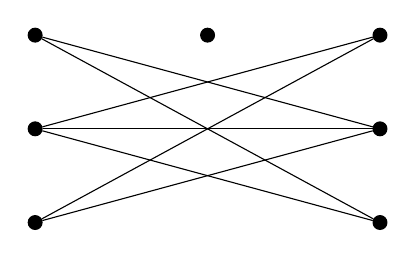
\begin{tikzpicture}[vertex/.style={circle,draw,fill=black,inner sep=0pt,minimum size=5pt}]
        \node[vertex] (a) {};
        \node[vertex] (b) [below=1cm of a] {};
        \node[vertex] (c) [below=1cm of b] {};
        \node[vertex] (g) [right=2cm of a] {};
        \node[vertex] (d) [right=2cm of g] {};
        \node[vertex] (e) [below=1cm of d] {};
        \node[vertex] (f) [below=1cm of e] {};

        \foreach \x in {e,f}{
            \draw (a)--(\x);
        }
        \foreach \x in {d,e,f}{
            \draw (b)--(\x);
        }
        \foreach \x in {d,e}{
            \draw (c)--(\x);
        }
    \end{tikzpicture}

    We can begin on the middle vertex, moving along \(C1\) until we reach a shared vertex.

    \begin{tikzpicture}[vertex/.style={circle,draw,fill=black,inner sep=0pt,minimum size=5pt}]
        \node[vertex] (a) {};
        \node[vertex] (b) [below=1cm of a] {};
        \node[vertex] (c) [below=1cm of b] {};
        \node[vertex] (g) [right=2cm of a] {};
        \node[vertex] (d) [right=2cm of g] {};
        \node[vertex] (e) [below=1cm of d] {};
        \node[vertex] (f) [below=1cm of e] {};

        \draw (g)--(a);
    \end{tikzpicture}

    At this point, we move over to \(C2\), tracing the entire cycle because there are no new cycles.

    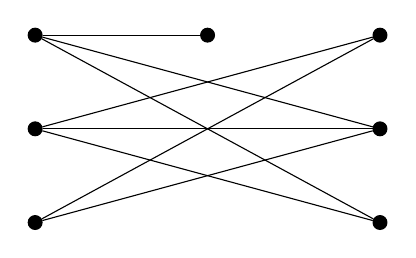
\begin{tikzpicture}[vertex/.style={circle,draw,fill=black,inner sep=0pt,minimum size=5pt}]
        \node[vertex] (a) {};
        \node[vertex] (b) [below=1cm of a] {};
        \node[vertex] (c) [below=1cm of b] {};
        \node[vertex] (g) [right=2cm of a] {};
        \node[vertex] (d) [right=2cm of g] {};
        \node[vertex] (e) [below=1cm of d] {};
        \node[vertex] (f) [below=1cm of e] {};

        \draw (g)--(a);
        \foreach \x in {e,f}{
            \draw (a)--(\x);
        }
        \foreach \x in {d,e,f}{
            \draw (b)--(\x);
        }
        \foreach \x in {d,e}{
            \draw (c)--(\x);
        }
    \end{tikzpicture}

    We are now back at the top left vertex, and complete tracing \(C1\). 

    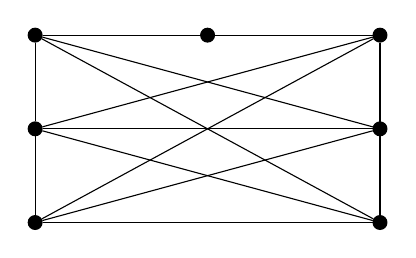
\begin{tikzpicture}[vertex/.style={circle,draw,fill=black,inner sep=0pt,minimum size=5pt}]
        \node[vertex] (a) {};
        \node[vertex] (b) [below=1cm of a] {};
        \node[vertex] (c) [below=1cm of b] {};
        \node[vertex] (g) [right=2cm of a] {};
        \node[vertex] (d) [right=2cm of g] {};
        \node[vertex] (e) [below=1cm of d] {};
        \node[vertex] (f) [below=1cm of e] {};

        \foreach \x in {b,d,e,f}{
            \draw (a)--(\x);
        }
        \foreach \x in {c,d,e,f}{
            \draw (b)--(\x);
        }
        \foreach \x in {d,e,f}{
            \draw (c)--(\x);
        }
        \draw (d)--(f);
    \end{tikzpicture}
\end{homeworkProblem}
\begin{homeworkProblem}
    Show that if \(G\) is not 2-connected, \(G\) is not Hamiltonian.
    \\

    \textbf{Solution}
    \\
    
    If \(G\) is not 2-connected, 
\end{homeworkProblem}
\end{document}
